%% ch05-quantum-learning.tex — Chapter IV (RQ2): Vectorized Encodings for Quantum Learning
%% Source papers: guo2025qpie, guo2025vqt, guo2025shardq, guo2026nnqa
%% Labels use the prefix qml: (sec:qml:*, fig:qml:*, tab:qml:*, eq:qml:*, alg:qml:*, thm:qml:*)
\chapter{Vectorized Encodings for Quantum Learning}\label{ch:qml}

This chapter addresses RQ2: how should classical data enter and leave a quantum processor so that learning models are shot-efficient, hardware-compatible and trainable? \Cref{ch:qgear} showed how far GPU simulation can push the development of quantum circuits. This chapter turns to learning, the layer on the classical--quantum boundary. Here the dominant cost is neither the simulator nor the optimizer (the subject of \cref{ch:nisq}) but the \emph{data interface}. The interface is the loader that turns a classical vector into a quantum state and the estimator that turns measurement counts back into numbers.

We argue that one family of \emph{vectorized} encodings yields learning primitives whose shot cost, gate count and trainability can be reasoned about in closed form. These encodings are uniformly controlled rotations on a data register indexed by an address register, in the lineage of \qcrank{} \cite{balewski2024qcrank}. Four systems substantiate the claim: \qpie{}, \vqt{}, \shardq{} and \nnqa{} (\cref{fig:qml:overview}).

\section{Introduction}\label{sec:qml:intro}

Most quantum algorithms with a provable advantage for linear algebra and learning make two assumptions. Examples are the linear-systems solver of Harrow, Hassidim and Lloyd \cite{harrow2009hhl}, the quantum singular value transformation \cite{gilyen2019qsvt}, and the kernel and principal-component methods surveyed by Biamonte et al.~\cite{biamonte2017qml}. They assume that the input is already available as a quantum state and that the output is a low-dimensional property of a quantum state. Neither assumption holds for a learning system that consumes classical images, sequences or tables and must return classical predictions.

Three costs follow. A generic amplitude encoding of $N$ real numbers costs $\Theta(N)$ two-qubit gates in the worst case. Tomography costs a number of shots that grows with the number of amplitudes to be resolved. The variational circuits usually placed between the two suffer from barren plateaus \cite{mcclean2018barren} as they grow. On a processor with a few hundred qubits and two-qubit error rates near $10^{-3}$ (\cref{sec:bg:nisq}), the data interface decides whether a quantum learning model can run at all. Accuracy is a later question.

This chapter takes the position that the interface should be \emph{structured} rather than generic. A vectorized encoding stores a classical value as the rotation angle of one data qubit, conditioned on an address register held in uniform superposition. So $n_d$ uniformly controlled rotations on $n_a$ address qubits load $N = 2^{n_a} n_d$ values, with $\Theta(N)$ CNOT gates in a fixed, hardware-friendly pattern \cite{mottonen2004ucr,balewski2024qcrank}.

Three consequences follow and recur throughout the chapter (\cref{fig:qml:overview}, top). First, every shot returns one address and one bit per data qubit, so all $N$ values are read out in parallel from the same shots. The shot cost is set by the precision required per value, not by the dimension of the Hilbert space. Second, the map from angles to expectation values is a product of cosines. Nonlinear computations on encoded values thus reduce to linear algebra over trigonometric quantities whose Jacobians are known classically. Gradients need not pass through the quantum processor. Third, the encoding, not an optimizer, fixes the circuit structure, so the compiler can cut, approximate and route the circuit with knowledge of the device.

The four contributions instantiate this position at increasing distance from conventional variational learning (\cref{fig:qml:overview}, bottom).
\begin{enumerate}
\item \qpie{} (\cref{sec:qml:qpie}) replaces the sequential stacking of a pretrained classical network and a variational quantum circuit by a \emph{parallel} exchange of information between them. It selects the gradient method at run time: the parameter-shift rule on a quantum processor, adjoint differentiation on a GPU simulator. It improves accuracy over classical transfer learning on the classification tasks with reported baselines, and it converges faster on two time-series tasks \cite{guo2025qpie}.
\item \vqt{} (\cref{sec:qml:vqt}) estimates the masked attention matrix of a transformer by a Vectorized Quantum Dot Product (VQDP). A Vectorized Nonlinear Quantum Encoder (VNQE) makes the encoding learnable. The quantum primitives run forward-only and need $\bigO{\log (BT^2)}$ qubits for a batch of $B$ sequences of length $T$. They were run on IBM and IonQ hardware with 4--9 qubits. The resulting language model is competitive with prior quantum transformers on the Brown corpus \cite{guo2025vqt}.
\item \shardq{} (\cref{sec:qml:shardq}) makes encodings that exceed the coherent depth budget of a superconducting device executable. It cuts them into sub-circuits with a deterministic, distance-ordered algorithm (SparseCut) and compiles the sub-circuits approximately as matrix-product states. It then recombines their outputs by a single global quasi-probability reconstruction. It lowers the reconstruction error of image encodings on IBM Heron processors by about 15\% relative to standard transpilation \cite{guo2025shardq}.
\item \nnqa{} (\cref{sec:qml:nnqa}) removes the variational loop from the quantum side altogether. A polynomial neural network is trained classically and compiled into exact quantum arithmetic built from weighted-sum and multiplication blocks on real-valued encoded states. It carries a universal-approximation guarantee. It reaches better than 99.5\% accuracy for polynomials up to degree 35 on IBM and IonQ hardware, in a single execution per polynomial \cite{guo2026nnqa}.
\end{enumerate}

% alt: Block diagram in two rows. Top row: a grey box for the address--data encoding feeds three blue boxes: parallel readout, products of cosines, and fixed gate pattern. Bottom row: four boxes for QPIE, VQT, ShardQ and NNQA sit from left to right above an arrow labelled less training on the quantum side; each box names its encoding, what the quantum processor does and where gradients are taken.
\begin{figure}[htbp]
\centering
\begin{tikzpicture}[
  font=\footnotesize,
  box/.style={draw,rounded corners=2pt,align=center,inner sep=3pt},
  prop/.style={box,fill=cbBlue!12,draw=cbBlue,text width=30mm,minimum height=8mm},
  met/.style={box,text width=26mm,minimum height=17mm},
  arr/.style={-{Stealth[length=2mm]},thick}]
\node[box,fill=cbGray!10,draw=cbGray,text width=32mm,minimum height=12mm] (enc) at (1.7,0) {\textbf{Address--data encoding}\\$N=2^{n_a}n_d$ values};
\node[prop] (p1) at (7.9,1.3) {Parallel readout};
\node[prop] (p2) at (7.9,0) {Classical Jacobians};
\node[prop] (p3) at (7.9,-1.3) {Cuttable gate pattern};
\draw[arr] (enc.east) -- ++(0.6,0) |- (p1.west);
\draw[arr] (enc.east) -- (p2.west);
\draw[arr] (enc.east) -- ++(0.6,0) |- (p3.west);
\node[met,fill=cbOrange!15,draw=cbOrange] (m1) at (0,-3.6) {\textbf{\qpie{}}\\angle encoding\\gradients on QPU or GPU};
\node[met,fill=cbGreen!12,draw=cbGreen] (m2) at (3.35,-3.6) {\textbf{\vqt{}}\\forward-only VQDP\\classical gradients};
\node[met,fill=cbPurple!15,draw=cbPurple] (m3) at (6.7,-3.6) {\textbf{\shardq{}}\\cut and knit\\no gradients};
\node[met,fill=cbRed!12,draw=cbRed] (m4) at (10.05,-3.6) {\textbf{\nnqa{}}\\exact arithmetic\\classical training};
\draw[arr,cbGray] (-1.7,-5.1) -- (11.75,-5.1);
\node[cbGray,anchor=north] at (5.0,-5.2) {less training on the quantum side};
\end{tikzpicture}
\caption{Overview of the chapter: the address--data encoding and its three properties (top), and the four methods ordered by how much training stays on the quantum side (bottom).}\label{fig:qml:overview}
\end{figure}

\Cref{sec:qml:prelim} fixes the notation for the address--data encoding and the design axes on which we compare methods. \Crefrange{sec:qml:qpie}{sec:qml:nnqa} present the four systems. \Cref{sec:qml:synthesis} compares them on common axes, states their shared design principles and limitations, and draws the bridges to \cref{ch:qgear,ch:nisq,ch:synthesis,ch:qec}. \Cref{sec:qml:summary} summarizes.

\section{Preliminaries: Vectorized Encodings and Design Axes}\label{sec:qml:prelim}

\Cref{sec:bg:encoding,sec:bg:cutting} give the general background on data encodings and circuit cutting. This section only fixes the notation of the chapter and the axes on which the four methods are compared.

\subsection{Address--Data Encodings}\label{sec:qml:prelim:ucr}

Let $\bm{x} \in [-1,1]^{N}$ be a real vector with $N = 2^{n_a} n_d$, indexed as $x_{k,j}$ with address $k \in \{0,\dots,2^{n_a}-1\}$ and data index $j \in \{1,\dots,n_d\}$. The \qcrank{} encoding \cite{balewski2024qcrank} prepares
\begin{equation}\label{eq:qml:qcrank}
\ket{\psi(\bm{x})} \;=\; \frac{1}{\sqrt{2^{n_a}}} \sum_{k=0}^{2^{n_a}-1} \ket{k}_A \otimes \bigotimes_{j=1}^{n_d} R_y(\theta_{k,j})\ket{0}_{D_j},
\qquad \theta_{k,j} = \arccos x_{k,j},
\end{equation}
by a layer of Hadamard gates on the address register $A$, followed by the uniformly controlled rotation (UCR) $U_j = \sum_k \ket{k}\!\bra{k} \otimes R_y(\theta_{k,j})$ for each data qubit $D_j$. Following Möttönen et al.~\cite{mottonen2004ucr}, $U_j$ is compiled into $2^{n_a}$ single-qubit $R_y$ rotations interleaved with $2^{n_a}$ CNOT gates. A Walsh--Hadamard transform of $\{\theta_{k,j}\}_k$ gives the rotation angles, and the CNOT controls follow a Gray-code sequence over the address qubits. The CNOT count is therefore exactly $n_d 2^{n_a} = N$ and the depth is $\bigO{2^{n_a}}$. The pattern is independent of the data, so it can be pre-compiled and, in \cref{sec:qml:shardq}, cut.

A measurement of all qubits in the computational basis yields, in each shot, an address $k$ and a bit $b_j$ for every data qubit. Conditioned on address $k$, $\Pr(b_j = 1 \mid k) = \sin^2(\theta_{k,j}/2) = (1 - x_{k,j})/2$. So with $S_k$ shots on address $k$ the estimator
\begin{equation}\label{eq:qml:readout}
\hat{x}_{k,j} \;=\; 1 - 2\hat{p}_{k,j}, \qquad
\operatorname{Var}\big(\hat{x}_{k,j} \mid S_k\big) \;=\; \frac{4\,p_{k,j}(1-p_{k,j})}{S_k} \;=\; \frac{1 - x_{k,j}^2}{S_k},
\end{equation}
is unbiased with binomial shot noise, where $p_{k,j} = \Pr(b_j = 1 \mid k)$. Because the address register is uniform, $S_k$ is multinomial with mean $S/2^{n_a}$ for $S$ shots in total. Every one of the $N$ values is estimated from the same run: the readout is \emph{quantum-parallel} in the sense of \cite{balewski2024qcrank}. We use $\eps$ for the target additive error per value, so $S = \bigO{2^{n_a}/\eps^2}$ shots suffice for all values simultaneously, up to logarithmic factors. \Cref{eq:qml:qcrank,eq:qml:readout} are the only two facts about the encoding that the rest of the chapter uses. \qcrank{} was demonstrated on trapped-ion and transmon devices in \cite{balewski2024qcrank}, its pixel-encoding predecessor QPIXL in \cite{amankwah2022qpixl}, and its relation to block encodings in \cite{camps2022fable}.

\subsection{Design Axes for Quantum Learning Primitives}\label{sec:qml:prelim:axes}

We compare the four methods on four axes that follow directly from RQ2.
\begin{itemize}
\item \emph{Where the nonlinearity lives.} A learning model needs nonlinear maps, and a quantum circuit is linear in the state. So the nonlinearity either comes from measurement statistics, as in conventional variational classifiers \cite{schuld2020circuitcentric,perezsalinas2020reuploading}, or sits in a classical layer around the circuit.
\item \emph{Trainability and gradient mechanism.} Are the quantum parameters trained at all? Are gradients taken through the quantum processor (parameter shift \cite{crooks2019parametershift}), through a simulator (adjoint differentiation \cite{jones2020adjoint}), or only through classical layers? Is the model exposed to barren plateaus \cite{mcclean2018barren}? Where a quantitative statement is possible, we use the spectrum of the empirical Fisher information matrix in the sense of Abbas et al.~\cite{abbas2021powerqnn}.
\item \emph{Shot scaling.} How does the total number of measurements grow with the size of the encoded data? For a vectorized encoding, \cref{eq:qml:readout} governs this growth.
\item \emph{Hardware compatibility.} How do the width and two-qubit depth of the compiled circuit compare with the coherence and connectivity of the device? Can the circuit be cut (\cref{sec:bg:cutting})?
\end{itemize}
\Cref{tab:qml:synthesis} in \cref{sec:qml:synthesis} records the position of each method on these axes.

\section{Non-Sequential Hybrid Networks: QPIE}\label{sec:qml:qpie}

\subsection{Motivation and Problem Statement}\label{sec:qml:qpie:motivation}

Quantum transfer learning after Mari et al.~\cite{mari2020transferlearning} stacks a pretrained classical feature extractor, a ``dressed'' variational quantum circuit and a classical classifier in sequence. The construction is attractive because the classical network absorbs the high-dimensional part of the input. But the sequential arrangement has three costs.
\begin{itemize}
\item The quantum layer lies on the critical path of every forward pass, so its shot cost and latency are paid on every sample.
\item The information that reaches the circuit passes through a bottleneck of a few features, one per qubit. So the pretrained parameters, which hold the transferred knowledge, never touch the quantum branch.
\item Every gradient of the loss with respect to a quantum parameter must be estimated from hardware or simulated. The cost grows with the number of parameters and with the number of shots per expectation value.
\end{itemize}
\qpie{} addresses these costs in two ways. It runs the classical and quantum branches in \emph{parallel} with an exchange of information between them. It also chooses the gradient estimator by the execution back-end \cite{guo2025qpie}.

\subsection{Architecture}\label{sec:qml:qpie:arch}

\Cref{fig:qml:qpie} sketches the architecture and one quantum block. The classical branch is a pretrained network $f_c(\bm{x}; \bm{W})$ whose parameters $\bm{W}$ may be frozen or fine-tuned. The quantum branch is a variational circuit $f_q(\bm{x}; \bm{\theta}, \bm{\varphi})$ built from blocks of ten data qubits and two ancilla qubits. The data qubits receive an angle encoding of (a projection of) $\bm{x}$. The trainable layers consist of parameterized single-qubit rotations of arbitrary angle interleaved with entangling gates. Such rotations are non-Clifford for generic angles, so the blocks lie outside the class that the Gottesman--Knill theorem renders efficiently simulable \cite{aaronson2004stabilizer}. This is a necessary (not sufficient) condition for the quantum branch to add expressivity.

The exchange is two-directional. A map $\bm{\varphi} = g(\bm{W})$ transfers pretrained classical parameters into rotation angles of the quantum block. The transferred knowledge is thus present in the circuit from the first training step. The expectation values of the block are concatenated with the classical features, and a fusion head $h$ produces the prediction,
\begin{equation}\label{eq:qml:qpie}
\hat{y} \;=\; h\big(f_c(\bm{x}; \bm{W}),\; f_q(\bm{x}; \bm{\theta}, g(\bm{W}))\big).
\end{equation}
In the reference implementation \cite{guo2025qpie} the classical branch is a pretrained ResNet-18 or ResNet-50 whose first two stages stay frozen. The map $g$ feeds the unlocked pretrained weights into the rotation angles of the variational gates. Up to 28 qubits cover about 45\% of the pretrained parameters. The rotation axis of each gate is chosen dynamically from the measured value $m$ of the preceding block: $R_x$ for $m<\tau_1$, $R_y$ for $\tau_1\le m<\tau_2$ and $R_z$ otherwise. The two ancilla qubits carry the exchange switch. The last qubit is measured, and its outcome (0 off, 1 on) decides whether the block exchanges information with the classical layer. The number of ancillas grows with the logarithm of the number of output classes.

In the topology of \cref{eq:qml:qpie} the branches are siblings, not stages, so the quantum block runs concurrently with the classical network. Pretrained information enters the circuit through parameters, not only through activations.

% alt: Two-panel figure. Panel (a) is a block diagram: an input feeds a pretrained classical network and, in parallel, a variational quantum circuit; a two-headed arrow labelled parameter exchange connects them; both outputs enter a fusion head that produces the prediction; a gradient selector box chooses parameter shift for QPU execution and adjoint differentiation for GPU simulation. Panel (b) is a circuit schematic with two ancilla wires and ten data wires (middle wires elided), showing angle-encoding rotations, a parameterized non-Clifford layer with CNOT entanglers, and measurements.
\begin{figure}[htbp]
\centering
\begin{subfigure}[b]{\linewidth}
\centering
\begin{tikzpicture}[
  font=\small,
  box/.style={draw,rounded corners=2pt,align=center,minimum height=10mm,inner sep=3pt},
  cls/.style={box,fill=cbBlue!12,draw=cbBlue},
  qua/.style={box,fill=cbOrange!15,draw=cbOrange},
  arr/.style={-{Stealth[length=2mm]},thick}]
\node[box,minimum width=16mm] (in) at (0,0) {Input $\bm{x}$};
\node[cls,text width=36mm] (c) at (4.4,1.5) {Pretrained classical\\network $f_c(\bm{x};\bm{W})$};
\node[qua,text width=36mm] (q) at (4.4,-1.5) {Variational quantum\\circuit $f_q(\bm{x};\bm{\theta},g(\bm{W}))$};
\node[box,text width=18mm] (h) at (9.2,0) {Fusion\\head $h$};
\node[box,minimum width=10mm] (out) at (11.6,0) {$\hat{y}$};
\node[box,fill=cbGray!10,text width=44mm] (gs) at (4.4,-3.6) {Gradient selector:\\QPU $\to$ parameter shift\\GPU $\to$ adjoint};
\draw[arr] (in.east) -- ++(0.7,0) |- (c.west);
\draw[arr] (in.east) -- ++(0.7,0) |- (q.west);
\draw[arr] (c.east) -- ++(1.4,0) |- (h.west);
\draw[arr] (q.east) -- ++(1.4,0) |- (h.west);
\draw[arr] (h) -- (out);
\draw[{Stealth[length=2mm]}-{Stealth[length=2mm]},thick,cbRed] (c.south) -- node[right,font=\footnotesize,align=center,xshift=1mm]{parameter exchange\\$\bm{\varphi}=g(\bm{W})$} (q.north);
\draw[arr,dashed] (gs) -- (q);
\end{tikzpicture}
\caption{Parallel information exchange between the classical and quantum branches.}\label{fig:qml:qpie:arch}
\end{subfigure}

\medskip
\begin{subfigure}[b]{\linewidth}
\centering
\begin{quantikz}[row sep={0.6cm,between origins},column sep=0.3cm,font=\small]
\lstick{$a_1$} & & \gate{R_y(\varphi_1)} & \ctrl{2} & & \meter{} \\
\lstick{$a_2$} & & \gate{R_y(\varphi_2)} & & \ctrl{1} & \meter{} \\
\lstick{$d_1$} & \gate{R_y(x_1)} & \gate{R_z(\theta_1)} & \targ{} & \targ{} & \meter{} \\
\lstick{$d_2$} & \gate{R_y(x_2)} & \gate{R_z(\theta_2)} & \ctrl{-1} & & \meter{} \\
\wave&&&&& \\
\lstick{$d_{10}$} & \gate{R_y(x_{10})} & \gate{R_z(\theta_{10})} & \ctrl{-2} & & \meter{}
\end{quantikz}
\caption{One quantum block (abbreviated): two ancilla and ten data qubits.}\label{fig:qml:qpie:block}
\end{subfigure}
\caption{The \qpie{} architecture. (a)~The pretrained classical branch and the variational quantum branch run in parallel and exchange information through the parameter map $g$ and the fusion head, and the gradient estimator is selected by the execution back-end. (b)~Schematic of one quantum block with two ancilla and ten data qubits; the wavy line elides seven data wires and the entangling pattern is indicative only. Schematic, after \cite{guo2025qpie}.}\label{fig:qml:qpie}
\end{figure}

\subsection{Dynamic Gradient Selection}\label{sec:qml:qpie:grad}

Let $E(\theta) = \expval{O}$ be an expectation value of a circuit whose dependence on $\theta$ enters through a gate $e^{-i\theta P/2}$ with $P^2 = I$. The parameter-shift rule \cite{crooks2019parametershift}
\begin{equation}\label{eq:qml:paramshift}
\frac{\partial E}{\partial \theta} \;=\; \tfrac{1}{2}\Big[E\big(\theta + \tfrac{\pi}{2}\big) - E\big(\theta - \tfrac{\pi}{2}\big)\Big]
\end{equation}
is exact and requires only expectation values, so it is the estimator of choice on hardware. Its cost is two circuit executions of $S$ shots per parameter, or $2PS$ shots per gradient for $P$ parameters. On a state-vector simulator the adjoint method \cite{jones2020adjoint} computes the whole gradient with one forward and one backward sweep over the state. Its cost is independent of $P$, up to the $\bigO{2^n}$ memory of the state. \qpie{} inspects the execution back-end at run time and selects \cref{eq:qml:paramshift} for quantum processors and adjoint differentiation for GPU simulators. Nothing else in the training loop changes.

The result reported in \cite{guo2025qpie} is a speed-up of up to $30\times$ for the GPU-simulated path over the CPU-simulated path. This made the 28-qubit configurations described next trainable. The containerized A100 workflow was the one developed for \qgear{} in \cref{ch:qgear}.

\subsection{Experimental Setup and Results}\label{sec:qml:qpie:results}

Experiments were run on the Amazon Braket SV1 state-vector simulator, on the IonQ Aria-1 trapped-ion processor and on local NVIDIA A100 GPUs. The circuits had up to 28 qubits built from blocks of ten data and two ancilla qubits \cite{guo2025qpie}. The implementation is a PyTorch model with the quantum blocks expressed in PennyLane, packaged as a container image. The image (a PennyLane Dockerfile and a PyTorch 24.06 Shifter image) targets an A100 with \SI{80}{GB} of memory for the adjoint-differentiated path. Seven tasks were used:
\begin{itemize}
\item the Moon and Spiral two-dimensional toy classification sets;
\item the Hymenoptera (ants versus bees) image set used in \cite{mari2020transferlearning};
\item a public brain-tumour MRI classification set;
\item MNIST \cite{lecun1998mnist};
\item the NARMA5 and NARMA10 nonlinear autoregressive time series \cite{atiya2000narma}.
\end{itemize}
The classical baseline is the corresponding classical transfer-learning model reported in the same paper. \Cref{tab:qml:qpie-results} collects the accuracies.

\begin{table}[htbp]
\caption{Classification accuracy of \qpie{} against the classical transfer-learning baseline, and convergence on stochastic time series. Ranges span the configurations reported in \cite{guo2025qpie}. Hymenoptera accuracies are not reproduced in the source summary used here and are omitted rather than estimated. Data from \cite{guo2025qpie}.}\label{tab:qml:qpie-results}
\centering
\small
\begin{tabular}{@{}llcc@{}}
\toprule
Task & Type & Classical baseline & \qpie{} \\
\midrule
Moon & 2-D toy, binary & 0.93 & 0.95--0.99 \\
Spiral & 2-D toy, binary & 0.90 & 0.96--0.99 \\
Hymenoptera & images, binary & --- & --- \\
Brain-tumour MRI & images, binary & 0.76 & 0.87--0.91 \\
MNIST & images, 10 classes & 0.81 & 0.93--0.97 \\
\midrule
NARMA5 / NARMA10 & time series & \multicolumn{2}{c}{$\approx$88\% faster convergence within 100 steps} \\
\bottomrule
\end{tabular}
\end{table}

Three further observations from \cite{guo2025qpie} bear on the design axes of \cref{sec:qml:prelim:axes}. First, on the two stochastic time-series tasks the parallel architecture converged roughly 88\% faster within a 100-step budget. We attribute this to the transferred parameters, which are present in the circuit from initialization and need not be learned through the activations. Second, the empirical Fisher information matrix of the \qpie{} model has a less biased spectrum than that of sequential transfer learning. The largest eigenvalues reach approximately 16 against approximately 7. In the framework of \cite{abbas2021powerqnn}, a Fisher spectrum less concentrated near zero means a larger effective dimension and less exposure to the vanishing gradients of \cite{mcclean2018barren}. We read it as evidence that the parameter exchange, not merely the added parameters, changes the geometry of the loss.

Third, the dynamic gradient selection delivered the GPU speed-up quoted above without any change to model code. This is the portability that RQ1 asked for and that \cref{ch:qgear} pursued at the simulator level.

\subsection{Discussion}\label{sec:qml:qpie:discussion}

The evidence for \qpie{} is strongest where the datasets are small and the baseline is a like-for-like transfer-learning model. It does not establish an advantage over state-of-the-art classical models on the same tasks, and the paper does not claim one. The contribution is architectural. The parallel placement of the quantum block removes it from the critical path and lets the compiler overlap its execution with the classical network. It also makes the choice of gradient estimator a property of the back-end, not of the model. The shot cost of \cref{eq:qml:paramshift} on hardware remains linear in the number of quantum parameters. This is the axis on which the remaining three systems move (\cref{fig:qml:overview}).

\section{Vectorized Attention: VQT}\label{sec:qml:vqt}

\subsection{From Attention to Dot Products}\label{sec:qml:vqt:attention}

The scaled dot-product attention of Vaswani et al.~\cite{vaswani2017attention} maps queries $Q$, keys $K$ and values $V$, each a $T \times d$ matrix per sequence, to
\begin{equation}\label{eq:qml:attention}
\operatorname{Attn}(Q,K,V) \;=\; \operatorname{softmax}\!\Big(\frac{QK^{\top}}{\sqrt{d}} + M\Big)\,V,
\end{equation}
where $M$ is the causal mask. For a batch of $B$ sequences the score matrix $QK^\top$ costs $\bigO{BT^2 d}$ multiply--adds and is the quadratic bottleneck of the architecture. Some previous quantum sequence models implement recurrent or attention layers as variational circuits, as in the quantum LSTM of Chen et al.~\cite{chen2022qlstm}. Others realise attention through linear combinations of unitaries and polynomial transformations of block encodings, as in Quixer \cite{khatri2024quixer}. Both place the trainable parameters inside the circuit.

\vqt{} takes a narrower view. The only quantum-native operation in \cref{eq:qml:attention} is the dot product. A $\tanh$ projection bounds the entries of $Q$ and $K$ to $[-1,1]$. A product of two bounded numbers is a product of two cosines. The vectorized encoding of \cref{eq:qml:qcrank} forms all $BT^2$ such products in one superposition \cite{guo2025vqt}.

\subsection{The Vectorized Quantum Dot Product}\label{sec:qml:vqt:vqdp}

Let $\mathcal{I}$ be the index set of the products $x_k y_k$ to be formed, enumerated by an address register of $n_a = \lceil \log_2 |\mathcal{I}| \rceil$ qubits. For the masked score matrix of a batch, $|\mathcal{I}|$ is proportional to $BT^2$, so $n_a = \bigO{\log(BT^2)}$. Two data qubits $D_Q$ and $D_K$ receive the UCRs with angles $\arccos x_k$ and $\arccos y_k$. A final CNOT from $D_Q$ to $D_K$ writes the parity $Z_Q Z_K$ onto $D_K$. In the product state conditioned on address $k$, $\expval{Z_Q Z_K}_k = \cos(\arccos x_k)\cos(\arccos y_k) = x_k y_k$, so the estimator
\begin{equation}\label{eq:qml:vqdp}
\hat{c}_k \;=\; 1 - 2\hat{p}_k, \qquad p_k = \Pr(b_K = 1 \mid k) = \frac{1 - x_k y_k}{2},
\end{equation}
is an unbiased estimate of the product. A score $a_{ts} = \sum_{i} q_{t,i} k_{s,i}$ is the sum of the $\hat{c}_k$ over the $d$ addresses that carry the pair $(t,s)$. The circuit has $2 \cdot 2^{n_a} + 1$ CNOT gates and two-qubit depth $2^{n_a} + 1$, and the hardware counts in \cref{tab:qml:vqt-hw} follow this formula exactly. The complexity reported in \cite{guo2025vqt} is $\bigO{\log(BT^2)\cdot \text{shots}}$ in qubits and executions against $\bigO{BT^2 d}$ classically. That is, the qubit count is logarithmic in the number of products, while the shot count, by \cref{eq:qml:readout}, is linear in it. We make the second half of that statement precise.

\begin{proposition}[Shot-noise variance of the VQDP estimator]\label{thm:qml:vqdp-variance}
Let the VQDP circuit on $n_a$ address qubits be executed $S$ times, let $S_k$ be the number of shots that return address $k$, and let $\hat{c}_k$ be the estimator of \cref{eq:qml:vqdp}. Then $\hat{c}_k$ is unbiased for $c_k = x_k y_k$ with
\begin{equation}\label{eq:qml:vqdp-var}
\operatorname{Var}\big(\hat{c}_k \mid S_k\big) \;=\; \frac{4\,p_k(1-p_k)}{S_k} \;=\; \frac{1 - c_k^2}{S_k} \;\le\; \frac{1}{S_k},
\end{equation}
and for a score $\hat{a} = \sum_{k \in \mathcal{I}_{ts}} \hat{c}_k$ over an index set of size $d$,
$\operatorname{Var}(\hat{a} \mid \{S_k\}) = \sum_{k \in \mathcal{I}_{ts}} (1 - c_k^2)/S_k$. In expectation over the uniform address distribution, $\mathbb{E}[S_k] = S/2^{n_a}$, so that $\operatorname{Var}(\hat{a}) \lesssim d\,2^{n_a}/S$ and $S = \bigO{d\,2^{n_a}/\eps^2}$ shots suffice for an additive error $\eps$ on every score simultaneously, up to logarithmic factors.
\end{proposition}

\begin{proof}[Proof sketch]
Conditioned on address $k$, the state of $D_K$ after the parity CNOT is a mixture whose $Z$-expectation is $c_k$, so each shot on address $k$ is a Bernoulli trial with success probability $p_k = (1 - c_k)/2$; the sample mean $\hat{p}_k$ of $S_k$ such trials has variance $p_k(1-p_k)/S_k$, which gives \cref{eq:qml:vqdp-var} after the affine map $\hat{c}_k = 1 - 2\hat{p}_k$. Shots on distinct addresses are independent, so variances add over $\mathcal{I}_{ts}$. The address register is prepared in the uniform superposition and is not acted on by the UCRs except as a control, so the address marginal is uniform and $S_k \sim \operatorname{Binomial}(S, 2^{-n_a})$; substituting the mean and applying a Chernoff bound to the deviation of $S_k$ from its mean yields the stated shot count. The full derivation, including the treatment of the multinomial fluctuation of $\{S_k\}$ and the constants under the paper's normalisation, is given in the appendix of \cite{guo2025vqt}; we have deliberately stated the bound without those constants.
\end{proof}

The proposition is both encouraging and sobering. The qubit count grows logarithmically and the two-qubit depth linearly in the number of products. But the shot budget grows linearly, as the operation count of a classical implementation does. The primitive is therefore not a route to an asymptotic speed-up of attention. Its value is that it is an \emph{executable} attention estimator on present hardware with an error known in closed form. Its Jacobian ($\partial (x_k y_k)/\partial x_k = y_k$) is classically available, so no gradient ever needs to be estimated on the quantum processor. This is the ``gradient-free'' property claimed in \cite{guo2025vqt}.

\subsection{Learnable Encoding: VNQE and the Two Attention Heads}\label{sec:qml:vqt:heads}

The second primitive addresses a weakness of fixed encodings identified by Schuld et al.~\cite{schuld2021encoding}: the encoding determines which functions the model can represent. The Vectorized Nonlinear Quantum Encoder (VNQE) makes the encoding learnable. A classical angle-learning layer, $\mathrm{Linear} \to \mathrm{GELU} \to \mathrm{Linear} \to \mathrm{ReLU}$ \cite{hendrycks2016gelu}, outputs the rotation angles of a small circuit. The circuit consists of a layer of Hadamard gates, a stack of \emph{expressive blocks} (parameterized $R_y$ and $R_z$ rotations followed by a CNOT ladder), and computational-basis measurements. The measured expectation values are the encoded features. \Cref{fig:qml:vnqe} shows the encoder next to the plain address--data encoder of \cref{eq:qml:qcrank} on which the VQDP is built.

% alt: Two circuit schematics. Panel (a): an address register of n_a qubits (drawn as a bundle) receives Hadamards and controls an R_y rotation on a data qubit, then all qubits are measured. Panel (b): three qubits receive Hadamards, then rotations R_y and R_z whose angles come from a classical MLP, then a CNOT ladder, a dashed box indicating repetition of the block L times, and measurements.
\begin{figure}[htbp]
\centering
\begin{subfigure}[b]{0.40\linewidth}
\centering
\begin{quantikz}[row sep={0.7cm,between origins},column sep=0.25cm,font=\footnotesize]
\lstick{$\ket{0}^{\otimes n_a}$} & \qwbundle{n_a} & \gate{H^{\otimes n_a}} & \ctrl{1} & \meter{} \\
\lstick{$\ket{0}_{D}$} & & & \gate{R_y(\theta_k)} & \meter{}
\end{quantikz}
\caption{Address--data encoder (UCR).}\label{fig:qml:vnqe:ucr}
\end{subfigure}\hfill
\begin{subfigure}[b]{0.58\linewidth}
\centering
\begin{quantikz}[row sep={0.6cm,between origins},column sep=0.18cm,font=\footnotesize]
\lstick{$\ket{0}$} & \gate{H} & \gate{R_y(\alpha_1)}\gategroup[3,steps=5,style={dashed,rounded corners,inner xsep=1pt},label style={label position=below,anchor=north,yshift=-0.15cm}]{{\footnotesize expressive block, $\times L$}} & \gate{R_z(\beta_1)} & \ctrl{1} & & \targ{} & \meter{} \\
\lstick{$\ket{0}$} & \gate{H} & \gate{R_y(\alpha_2)} & \gate{R_z(\beta_2)} & \targ{} & \ctrl{1} & & \meter{} \\
\lstick{$\ket{0}$} & \gate{H} & \gate{R_y(\alpha_3)} & \gate{R_z(\beta_3)} & & \targ{} & \ctrl{-2} & \meter{}
\end{quantikz}
\caption{VNQE layer; angles $(\bm\alpha,\bm\beta)=\mathrm{MLP}(\bm{x})$.}\label{fig:qml:vnqe:layer}
\end{subfigure}
\caption{Encoders used in \vqt{}. (a)~The address--data encoder of \cref{eq:qml:qcrank}, with the address register drawn as a bundle; the VQDP uses two such data qubits and a parity CNOT. (b)~The Vectorized Nonlinear Quantum Encoder: a classical layer $\mathrm{Linear}\to\mathrm{GELU}\to\mathrm{Linear}\to\mathrm{ReLU}$ produces the rotation angles of a Hadamard layer followed by $L$ expressive blocks; measured expectation values are the encoded features. Schematic, after \cite{guo2025vqt}.}\label{fig:qml:vnqe}
\end{figure}

The two primitives are assembled into two attention heads (\cref{fig:qml:vqt-heads}). The \emph{tanh projection head} applies $\tanh$ projections to $Q$, $K$ and $V$ and estimates the score matrix by the VQDP. The values receive a further $\tanh$ projection. A masked attention layer then performs the softmax and the multiplication by $V$ classically. The \emph{expressive quantum head} replaces the $\tanh$ projections by angle MLPs and inserts a VNQE between the VQDP and the masked attention layer. In both heads all trainable parameters sit in classical layers, and the VQDP is a fixed map with a classically known Jacobian. So back-propagation never requires a parameter-shift evaluation on the quantum processor.

During training the quantum primitives were evaluated by shot-based simulation on Perlmutter GPU nodes. The expressive block is not differentiated at all. The angle MLP in front of the VNQE is the only trainable part, and the circuit outputs enter the loss as fixed features. The workflow is therefore gradient-free on the quantum side \cite{guo2025vqt}, and the hardware runs reported below are inference-only.

% alt: Two horizontal pipelines. Top, labelled tanh projection head: Q/K/V tanh projections, then VQDP, then value tanh projection, then masked attention layer, then output. Bottom, labelled expressive quantum head: Q/K/V angle MLPs, then VQDP, then VNQE, then masked attention layer, then output. Quantum stages are shaded orange, classical stages blue.
\begin{figure}[htbp]
\centering
\begin{tikzpicture}[
  font=\footnotesize,
  box/.style={draw,rounded corners=2pt,align=center,minimum height=8mm,text width=19mm,inner sep=2pt},
  cls/.style={box,fill=cbBlue!12,draw=cbBlue},
  qua/.style={box,fill=cbOrange!15,draw=cbOrange},
  arr/.style={-{Stealth[length=2mm]},thick},
  node distance=4mm]
\node[font=\small\bfseries,anchor=west] (t1) at (0,1.1) {Tanh projection head};
\node[cls,anchor=west] (a1) at (0,0) {$\tanh$ projections};
\node[qua,right=of a1] (a2) {VQDP};
\node[cls,right=of a2] (a3) {value projection};
\node[cls,right=of a3] (a4) {attention};
\node[right=of a4] (a5) {out};
\draw[arr] (a1)--(a2); \draw[arr] (a2)--(a3); \draw[arr] (a3)--(a4); \draw[arr] (a4)--(a5);
\node[font=\small\bfseries,anchor=west] (t2) at (0,-1.4) {Expressive quantum head};
\node[cls,anchor=west] (b1) at (0,-2.5) {angle MLPs};
\node[qua,right=of b1] (b2) {VQDP};
\node[qua,right=of b2] (b3) {VNQE};
\node[cls,right=of b3] (b4) {attention};
\node[right=of b4] (b5) {out};
\draw[arr] (b1)--(b2); \draw[arr] (b2)--(b3); \draw[arr] (b3)--(b4); \draw[arr] (b4)--(b5);
\node[cls,minimum height=4mm,text width=12mm,anchor=west] (l1) at (0,-3.7) {classical};
\node[qua,minimum height=4mm,text width=12mm,right=2mm of l1] (l2) {quantum};
\end{tikzpicture}
\caption{The two attention heads of \vqt{}. Orange stages run on the quantum processor forward-only; blue stages are classical and hold all trainable parameters. Schematic, after \cite{guo2025vqt}.}\label{fig:qml:vqt-heads}
\end{figure}

\subsection{Hardware Evaluation of the VQDP}\label{sec:qml:vqt:hw}

The VQDP was benchmarked as a micro-kernel on an ideal simulator, the IBM Kingston superconducting processor and the IonQ Aria-1 trapped-ion processor \cite{guo2025vqt}. Each address held one query--key product pair. The batch sizes were 4 to 128, with $n_a = 2$ to $7$ address qubits plus the two data qubits. The total shot count grew from 10K to 320K with the batch size. The circuits were generated by the \texttt{quantum-transformer} code base and submitted to IonQ through its job API and to IBM through \qiskit{}. The figure-reproduction scripts and raw hardware data are published with the paper, and the arithmetic identities behind the VQDP were checked symbolically in Mathematica. \Cref{tab:qml:vqt-hw} lists the circuit statistics and the root-mean-square error (RMSE) of the estimated products against their exact values, and \cref{fig:qml:vqt-rmse} plots the RMSE.

\begin{table}[htbp]
\caption{VQDP micro-kernel on an ideal simulator, IBM Kingston and IonQ Aria-1: circuit statistics after compilation and RMSE of the estimated products. Qubit counts include two data qubits. Total shots grow from 10K (batch 4) to 320K (batch 128). A dash marks a configuration that was not run or did not return a usable result. Data from \cite{guo2025vqt}.}\label{tab:qml:vqt-hw}
\centering
\footnotesize
\begin{tabular}{@{}rr rrr rrr r@{}}
\toprule
& & \multicolumn{3}{c}{Ideal simulator} & \multicolumn{3}{c}{IBM Kingston} & Aria-1 \\
\cmidrule(lr){3-5}\cmidrule(lr){6-8}\cmidrule(l){9-9}
Batch & Qubits & \#CX & CX depth & RMSE & \#CZ & CZ depth & RMSE & RMSE \\
\midrule
4   & 4 & 9   & 5   & 0.017 & 18  & 14  & 0.022 & 0.057 \\
8   & 5 & 17  & 9   & 0.016 & 29  & 25  & 0.023 & 0.155 \\
16  & 6 & 33  & 17  & 0.017 & 78  & 69  & 0.037 & 0.215 \\
32  & 7 & 65  & 33  & 0.017 & 164 & 121 & 0.059 & --- \\
64  & 8 & 129 & 65  & 0.016 & 348 & 249 & 0.274 & --- \\
128 & 9 & 257 & 129 & 0.016 & 704 & 514 & ---   & --- \\
\bottomrule
\end{tabular}
\end{table}

% alt: Line chart of RMSE against batch size on a base-2 logarithmic horizontal axis. The ideal-simulator series is flat near 0.017 for all batch sizes 4 to 128. The IBM Kingston series rises slowly from 0.022 at batch 4 to 0.059 at batch 32 and then jumps to 0.274 at batch 64. The IonQ Aria-1 series rises from 0.057 at batch 4 to 0.215 at batch 16.
\begin{figure}[htbp]
\centering
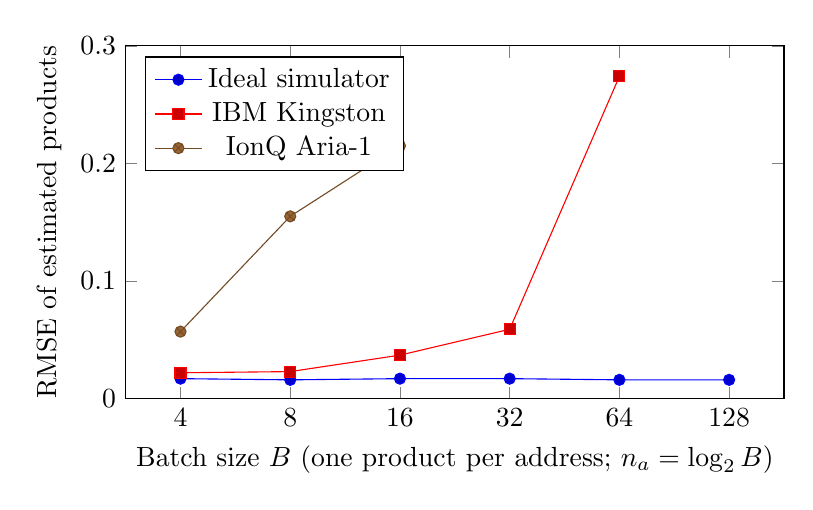
\begin{tikzpicture}
\begin{axis}[
  xmode=log, log basis x=2,
  xlabel={Batch size $B$ (one product per address; $n_a=\log_2 B$)},
  ylabel={RMSE of estimated products},
  xtick={4,8,16,32,64,128},
  xticklabels={4,8,16,32,64,128},
  ymin=0, ymax=0.30,
  legend pos=north west,
  width=0.82\linewidth,height=0.5\linewidth]
\addplot coordinates {(4,0.017) (8,0.016) (16,0.017) (32,0.017) (64,0.016) (128,0.016)};
\addlegendentry{Ideal simulator}
\addplot coordinates {(4,0.022) (8,0.023) (16,0.037) (32,0.059) (64,0.274)};
\addlegendentry{IBM Kingston}
\addplot coordinates {(4,0.057) (8,0.155) (16,0.215)};
\addlegendentry{IonQ Aria-1}
\end{axis}
\end{tikzpicture}
\caption{RMSE of the VQDP estimate of the products $x_k y_k$ versus batch size on the ideal simulator, IBM Kingston and IonQ Aria-1. Re-plotted from the values reported in \cite{guo2025vqt}; all plotted points are the reported values.}\label{fig:qml:vqt-rmse}
\end{figure}

Three features of the data stand out. First, the ideal-simulator RMSE is flat at 0.016--0.017 across a $32\times$ range of batch sizes. This is what \cref{thm:qml:vqdp-variance} predicts when the total shot count grows in proportion to $2^{n_a}$, so that the shots per address stay constant.

Second, on IBM Kingston the compiled circuit has roughly two to three times the two-qubit gates of the ideal circuit and a proportionally larger depth. The cause is the routing of the star-shaped address--data connectivity of the UCR onto the heavy-hexagonal coupling map. The RMSE follows the depth. It grows gently from 0.022 to 0.059 up to a CZ depth of 121 and then jumps to 0.274 at depth 249. No result is reported at batch 128. Third, on IonQ Aria-1 the all-to-all connectivity needs no routing, but the two-qubit gates are slower. There the RMSE grows from 0.057 at batch 4 to 0.215 at batch 16, and no results are reported for larger batches.

The paper also shows the reconstructed products as a scatter plot of $\hat{c}_k$ against the exact $x_k y_k$. On the simulator the points lie on the diagonal with a width consistent with \cref{eq:qml:vqdp-var}. On hardware the cloud both widens and contracts toward zero as depth grows, the signature of depolarizing noise that shrinks the parity expectation. At the level of the full attention matrix, the quantum estimate deviated from the classical one by less than 1.2\% with $3.0$M shots \cite{guo2025vqt}.

\subsection{Language Modelling on the Brown Corpus}\label{sec:qml:vqt:lm}

To test the primitives inside a complete model, \vqt{} was trained as a small autoregressive language model on the Brown corpus \cite{francis1979brown}. It was compared with a 125K-parameter nanoGPT \cite{karpathy2023nanogpt} and with three published quantum sequence models. These are the quantum LSTM of Chen et al.~\cite{chen2022qlstm}, Quixer \cite{khatri2024quixer} and the hybrid quantum transformer of Smaldone et al.~\cite{smaldone2025hybridqt}. \Cref{tab:qml:vqt-lm} reproduces the comparison.

\begin{table}[htbp]
\caption{Language modelling on the Brown corpus: perplexity (reported as QPL in \cite{guo2025vqt}) and cross-entropy loss. Lower is better for both. Parameter and qubit counts as reported; a dash means the value was not reported in the source summary. Data from \cite{guo2025vqt}.}\label{tab:qml:vqt-lm}
\centering
\small
\begin{tabular}{@{}llrrrr@{}}
\toprule
Model & Year & Qubits & Parameters & Perplexity & Loss \\
\midrule
nanoGPT \cite{karpathy2023nanogpt} & 2023 & --- & 125K & 92.5 & 0.94 \\
Q-LSTM \cite{chen2022qlstm} & 2022 & 6 & --- & 125.3 & 1.18 \\
Quixer \cite{khatri2024quixer} & 2024 & --- & --- & 117.1 & 1.61 \\
Hybrid quantum transformer & 2025 & --- & --- & 127.6 & 1.08 \\
\vqt{}, default & 2025 & 6 & --- & 105.4 & 1.12 \\
\vqt{}, large encoder & 2025 & 12 & --- & 108.2 & 1.08 \\
\bottomrule
\end{tabular}
\end{table}

The default \vqt{} configuration with six qubits reaches a perplexity of 105.4 and a loss of 1.12. This beats all three quantum baselines on perplexity. It is within about 14\% of the classical nanoGPT, which has no quantum bottleneck and roughly 125K trainable parameters. A larger encoder with twelve qubits lowers the loss to 1.08 but raises the perplexity slightly to 108.2. The two metrics are reported separately in \cite{guo2025vqt}, and we read no more into the difference than that the larger encoder does not uniformly help. The comparison is fair in that all quantum models are evaluated on the same corpus. But the baselines were trained under their own published protocols, so the table supports a claim of competitiveness, not of dominance.

\subsection{Discussion}\label{sec:qml:vqt:discussion}

\vqt{} demonstrates the second design principle of the chapter. Nonlinearity and trainability stay on the classical side, and the quantum processor performs a fixed, vectorized, forward-only computation whose error is understood.

The binding constraint that emerged from the hardware evaluation is two-qubit depth. The UCR depth $2^{n_a}$ doubles with each address qubit, and on a heavy-hex device the routed depth is two to four times larger still. \Cref{tab:qml:vqt-hw} locates the failure point of the 2025 IBM Kingston processor between a CZ depth of 121 and 249. Another factor of four in the encoded data therefore needs better hardware or a compiler that divides the encoding into pieces the hardware can execute. \shardq{} is that compiler.

\section{Hardware-Aware Circuit Knitting for Encodings: ShardQ}\label{sec:qml:shardq}

\subsection{Problem: Encodings That Do Not Fit}\label{sec:qml:shardq:problem}

A 1,000-pixel grey-scale image encoded by \cref{eq:qml:qcrank} needs $n_a = 9$ address and $n_d = 2$ data qubits, $2 \times 512$ CNOT gates before routing, and a two-qubit depth of the order of 512. This is well beyond what \cref{tab:qml:vqt-hw} showed to be executable. Circuit cutting offers a way out.

A two-qubit gate can be replaced by a quasi-probability decomposition (QPD) into local operations on its two qubits \cite{mitarai2021virtualgate,peng2020circuitcutting,bravyi2016trading}. For a CNOT or CZ gate, $U = \sum_i c_i A_i \otimes B_i$ with $\sum_i |c_i| = \gamma = 3$. Any expectation value of the original circuit is then recovered as a signed combination of expectation values of the two disconnected sub-circuits. The sampling overhead is $\gamma^2 = 9$ per cut and hence $\bigO{3^{2k}}$ for $k$ cuts.

Classical communication between sub-circuits can reduce the overhead \cite{piveteau2024knitting}, and general-purpose cutters such as CutQC \cite{tang2021cutqc} choose where to cut by partitioning the circuit graph. None of these methods looks at the device. The premise of \shardq{} has two parts \cite{guo2025shardq}. First, for an encoding circuit whose structure is fixed by \cref{eq:qml:qcrank}, the address--data structure of the encoder itself determines the right place to cut. The gates that span the longest virtual-qubit distance cost most on a device with limited connectivity. Second, the sub-circuits are encodings themselves, so they have low entanglement and can be compiled approximately.

\subsection{SparseCut: Deterministic Cut Selection by Entanglement Distance}\label{sec:qml:shardq:sparsecut}

SparseCut, given in \cref{alg:qml:sparsecut}, works on the address--data structure of the encoder, not on a generic circuit graph. It collects every two-qubit gate that couples an address qubit $q_i\in A$ to a data qubit $q_j\in D$ and scores each such gate by the virtual-qubit distance
\begin{equation}\label{eq:qml:sparsecut-score}
d(g) \;=\; \lvert i - j\rvert,
\end{equation}
and then sorts the candidates by $d$ in descending order. It returns the first $\min(\lvert G_{\mathrm{cross}}\rvert, k_{\max})$ of them as cuts. The hyper-parameter $k_{\max}$ (\texttt{max\_cuts} in \cite{guo2025shardq}) bounds the $3^{2k}$ sampling overhead the user is willing to pay.

The rule cuts the longest entanglement distances first, which follows the Gray-code structure of the encoder. There, the gates that span the most qubits are the ones that routing on a heavy-hex device would pay for most. The absolute distance makes the rule independent of the bit ordering of the platform. The dominant cost is the sort, $\bigO{|G| \log |G|}$ for $|G|$ gates. The procedure is deterministic: the same circuit and the same cut budget always give the same cuts.

The device enters through the transpilation of the sub-circuits and through the noise model of the experiments. The noise model was derived from the calibration snapshot of \texttt{ibm\_pittsburgh} (median CZ error $1.46\times10^{-3}$, median $\sqrt{X}$ error $1.62\times10^{-4}$) \cite{guo2025shardq}. Graph-partitioning cutters minimize the number of cut edges. SparseCut instead prefers to cut the gates that would be \emph{most expensive} to execute, even if that means one more cut.

\begin{algorithm}[htbp]
\caption{SparseCut: deterministic cut selection for address--data encoders (after Alg.~1 of \cite{guo2025shardq}).}\label{alg:qml:sparsecut}
\KwIn{Encoding circuit $C$; address qubit set $A$; data qubit set $D$; cut budget $k_{\max}$.}
\KwOut{Cut set $\mathcal{C}$ of two-qubit gates to replace by QPD cuts.}
$G_{\mathrm{cross}} \leftarrow \emptyset$\;
\ForEach{two-qubit gate $g=(q_i,q_j)$ in $C$}{
  \If{$(q_i\in A \wedge q_j\in D) \vee (q_i\in D \wedge q_j\in A)$}{
    $d \leftarrow \lvert i-j\rvert$\;
    $G_{\mathrm{cross}} \leftarrow G_{\mathrm{cross}} \cup \{(g, d)\}$\;
  }
}
sort $G_{\mathrm{cross}}$ by $d$ in descending order \tcp*{$\bigO{|G|\log|G|}$}
\Return{the first $\min(\lvert G_{\mathrm{cross}}\rvert, k_{\max})$ gates of $G_{\mathrm{cross}}$ as $\mathcal{C}$}
\end{algorithm}

\subsection{MPS Approximate Compilation and Global Reconstruction}\label{sec:qml:shardq:mps}

Each sub-circuit produced by SparseCut is itself an address--data encoding on a subset of the qubits. Its output state is a uniform superposition over a smaller address register with product-state data qubits attached. So the entanglement across any bipartition is bounded by the size of the address subregister. The state admits a matrix-product-state (MPS) representation \cite{vidal2003mps,perezgarcia2006mps} of modest bond dimension.

\shardq{} exploits this and compiles each sub-circuit \emph{approximately}. The target state is written as an MPS with bond dimension truncated to a bound $\chi$. A shallower circuit that prepares the truncated MPS replaces the original. The discarded Schmidt weights control the truncation error, which trades against depth. The classical side of the pipeline, MPS compilation and the reconstruction described next, runs on GPUs. Configurations with up to two cuts take about \SI{15}{\second} on one \SI{80}{GB} A100. Four cuts, whose reconstruction involves $3^{8}$ QPD terms, occupied four GPU nodes for about \SI{24}{\hour} \cite{guo2025shardq}.

A \emph{global} quasi-probability reconstruction recombines the outputs of the sub-circuits. With $k$ cuts indexed by $i_1,\dots,i_k$ and QPD coefficients $c^{(m)}_{i_m}$, the expectation of an observable $O$ on the uncut circuit is
\begin{equation}\label{eq:qml:qpd}
\expval{O} \;=\; \sum_{i_1,\dots,i_k} \Big(\prod_{m=1}^{k} c^{(m)}_{i_m}\Big)\; \expval{O}_{\text{sub-circuits}(i_1,\dots,i_k)},
\end{equation}
where the right-hand expectation is a product over the sub-circuits of expectation values taken with the local operations selected by the indices. Pairwise knitting evaluates \cref{eq:qml:qpd} one cut at a time: it recombines two sub-circuits into a virtual larger one and repeats. Each stage introduces its own finite-sample error, and the errors compound.

\shardq{} instead forms the full sum over the joint index set once, from the measured distributions of all sub-circuits. The reconstruction error is then that of a single estimator, not of a chain of them. The price is the $3^{2k}$ sampling overhead, which the GPU absorbs. \Cref{fig:qml:shardq} summarizes the pipeline.

% alt: Three-stage pipeline diagram. Left: a wide encoding circuit with address and data wires, crossed by two red dashed cut lines through two-qubit gates. Middle: three smaller sub-circuit boxes, each labelled with a hardware region and its calibrated CZ error, each annotated as MPS-compiled with bond dimension chi. Right: a box labelled global QPD reconstruction summing over all cut indices, producing the reconstructed data values.
\begin{figure}[htbp]
\centering
\begin{tikzpicture}[
  font=\footnotesize,
  box/.style={draw,rounded corners=2pt,align=center,inner sep=3pt},
  arr/.style={-{Stealth[length=2mm]},thick},
  node distance=6mm]
% stage 1: full circuit
\node[box,minimum width=30mm,minimum height=26mm,fill=cbBlue!8,draw=cbBlue] (full) at (0,0) {};
\node[above=1mm of full.north,font=\footnotesize\bfseries,align=center,text width=34mm] {Encoding circuit\\($n_a{+}n_d$ qubits)};
\foreach \y in {9,6,3,0,-3,-6} {\draw ($(full.west)+(1mm,\y mm)$) -- ($(full.east)+(-1mm,\y mm)$);}
\foreach \x in {-10,-4,2,8} {\draw[fill=white] ($(full.center)+(\x mm,4.5mm)$) circle (0.9mm);}
\foreach \x in {-7,-1,5,11} {\draw[fill=white] ($(full.center)+(\x mm,-1.5mm)$) circle (0.9mm);}
\draw[cbRed,dashed,very thick] ($(full.center)+(-5.5mm,-12mm)$) -- ($(full.center)+(-5.5mm,11mm)$);
\draw[cbRed,dashed,very thick] ($(full.center)+(6.5mm,-12mm)$) -- ($(full.center)+(6.5mm,11mm)$);
\node[cbRed,font=\scriptsize] at ($(full.center)+(-5.5mm,-10mm)$) [fill=white,inner sep=1pt] {cut 1};
\node[cbRed,font=\scriptsize] at ($(full.center)+(6.5mm,-10mm)$) [fill=white,inner sep=1pt] {cut 2};
\node[below=1mm of full.south,text width=34mm,align=center] {SparseCut: score gates by distance $+$ calibrated error};
% stage 2: sub-circuits
\node[box,fill=cbOrange!12,draw=cbOrange,text width=27mm,minimum height=9mm] (s1) at (4.8,1.4) {sub-circuit 1\\region $R_1$, $\eps_2(R_1)$};
\node[box,fill=cbOrange!12,draw=cbOrange,text width=27mm,minimum height=9mm] (s2) at (4.8,0.0) {sub-circuit 2\\region $R_2$, $\eps_2(R_2)$};
\node[box,fill=cbOrange!12,draw=cbOrange,text width=27mm,minimum height=9mm] (s3) at (4.8,-1.4) {sub-circuit 3\\region $R_3$, $\eps_2(R_3)$};
\node[above=1mm of s1.north,font=\footnotesize\bfseries,align=center,text width=36mm] {MPS-compiled,\\bond dimension $\le\chi$};
\node[below=1mm of s3.south,text width=32mm,align=center] {$3^{k}$ QPD variants each;\\$1.5$M shots per sub-circuit};
% stage 3: reconstruction
\node[box,fill=cbGreen!12,draw=cbGreen,text width=32mm,minimum height=16mm] (rec) at (9.5,0) {Global QPD reconstruction\\[3pt]$\sum_{\bm{i}}\prod_{m} c^{(m)}_{i_m}\,\expval{O}_{\bm{i}}$};
\node[above=1mm of rec.north,font=\footnotesize\bfseries] {Knit once (GPU)};
\node[box,right=3mm of rec,text width=19mm,minimum height=10mm] (out) {reconstructed\\values $\hat{\bm{x}}$};
\draw[arr] (full.east) -- (s1.west);
\draw[arr] (full.east) -- (s2.west);
\draw[arr] (full.east) -- (s3.west);
\draw[arr] (s1.east) -- (rec.west);
\draw[arr] (s2.east) -- (rec.west);
\draw[arr] (s3.east) -- (rec.west);
\draw[arr] (rec) -- (out);
\end{tikzpicture}
\caption{The \shardq{} pipeline. SparseCut selects gate cuts of the encoding circuit from physical qubit distance and calibrated two-qubit error; each sub-circuit is compiled approximately as a matrix-product state of bounded bond dimension and executed on a well-calibrated region of the processor; all sub-circuit outputs are recombined by a single global quasi-probability reconstruction. Schematic, after \cite{guo2025shardq}.}\label{fig:qml:shardq}
\end{figure}

\subsection{Experimental Setup and Results}\label{sec:qml:shardq:results}

Experiments were run on two IBM Heron processors. \texttt{ibm\_pittsburgh} is a Heron r3 device whose median CZ error was $\num{1.46e-3}$ at the time of the runs. \texttt{ibm\_marrakesh} is a Heron r2 device. The encodings had 2--9 address and 2--8 data qubits, including 1,000-pixel images at 9 address and 2 data qubits. Each sub-circuit received $1.5$M shots \cite{guo2025shardq}. The implementation (\texttt{ShardQ\_v2}) has four parts:
\begin{itemize}
\item the \qiskit{} circuit-cutting add-on for the QPD primitives;
\item the device calibration (two-qubit error, $T_1$, $T_2$), read through the \qiskit{} runtime;
\item MPS simulation and compilation on GPUs for circuits beyond 100 qubits;
\item CutQC-style and random cut selection as baselines for SparseCut.
\end{itemize}
The baseline for the hardware comparison was the same encoding transpiled by the standard \qiskit{} pipeline and executed uncut. Reconstruction quality was measured by the RMSE between reconstructed and true values and by a fidelity of the reconstructed value vector.

Across the configurations the cut-and-knit pipeline reduced the RMSE by roughly 15\% relative to standard transpilation. For image encodings the fidelity rose from 0.79 for the uncut \qcrank{} circuit to 0.90 with \shardq{} at five address qubits, and from 0.75 to 0.88 at seven address qubits. As expected, the gap widens with the number of address qubits: the uncut depth doubles, while the sub-circuit depth stays near the device budget. \Cref{tab:qml:shardq-overhead} records the sampling overhead and the classical cost against the number of cuts.

\begin{table}[htbp]
\caption{Sampling overhead and classical (GPU) cost of \shardq{} versus the number of gate cuts $k$. The overhead column is the QPD variance factor $\gamma^{2k} = 3^{2k}$ for CZ/CNOT cuts; GPU resources and wall-clock times for MPS compilation plus reconstruction are those reported in \cite{guo2025shardq}; a dash marks a configuration not reported.}\label{tab:qml:shardq-overhead}
\centering
\small
\begin{tabular}{@{}crrll@{}}
\toprule
Cuts $k$ & QPD terms $3^{k}$ & Overhead $3^{2k}$ & GPU resources & Wall-clock \\
\midrule
0 & 1 & 1 & --- (uncut baseline) & --- \\
1 & 3 & 9 & one A100 (\SI{80}{GB}) & $\approx$\SI{15}{\second} \\
2 & 9 & 81 & one A100 (\SI{80}{GB}) & $\approx$\SI{15}{\second} \\
3 & 27 & 729 & --- & --- \\
4 & 81 & 6\,561 & four GPU nodes & $\approx$\SI{24}{\hour} \\
\bottomrule
\end{tabular}
\end{table}

\subsection{Discussion}\label{sec:qml:shardq:discussion}

The result is a compiler result, not an error-mitigation result: no additional shots are spent on mitigation, and no noise model is inverted. The gain comes from shorter circuits on better couplers, paid for with classical resources: MPS compilation and a global reconstruction on GPUs. The exponential overhead in \cref{tab:qml:shardq-overhead} is the honest limit of the method. Two cuts are cheap, four cuts cost a day on four GPU nodes, and six would be out of reach.

The approach therefore suits encodings that are a small constant factor too deep for the device, exactly the regime that \cref{tab:qml:vqt-hw} identified for the VQDP. It also exemplifies the third principle of the chapter, that the compiler should know the device. SparseCut consumes the same calibration data that \cref{ch:qec} will treat as a security-relevant fault map, a connection we return to in \cref{sec:qml:synthesis:bridges}.

\section{Neural-Native Quantum Arithmetic: NNQA}\label{sec:qml:nnqa}

\subsection{Motivation}\label{sec:qml:nnqa:motivation}

The three systems so far keep some computation variational or approximate on the quantum side. \nnqa{} asks whether that is necessary at all for a large and useful class of functions. A polynomial neural network has polynomial activations, so the whole network is a multivariate polynomial of bounded degree. Such a network can be trained with ordinary classical machinery. A polynomial is exactly the function class that quantum arithmetic on real-valued encoded states can evaluate. The EHands protocol of Balewski et al.~\cite{balewski2025ehands} showed how to add, scale and multiply values stored as rotation angles in the \qcrank{} convention.

\nnqa{} builds on that lineage. It compiles the trained network into a fixed circuit of native unitary blocks that evaluates the polynomial \emph{exactly} in the ideal expectation. No optimizer runs on the quantum side, and each input needs a single execution \cite{guo2026nnqa}. It displaces two alternatives. The variational quantum eigensolver family \cite{peruzzo2014vqe,cerezo2021vqa} pays $10^2$--$10^3$ executions for the optimization loop. Quantum signal processing \cite{low2017qsp,gilyen2019qsvt} evaluates polynomials of a block-encoded operator at a depth proportional to the degree and with ancilla overhead.

\subsection{Arithmetic Blocks on Real-Valued Encoded States}\label{sec:qml:nnqa:blocks}

A real value $x \in [-1,1]$ is stored as $R_y(\arccos x)\ket{0}$, so that $\expval{Z} = x$. Two blocks suffice for polynomials. The \emph{multiplication} block places $m$ such qubits side by side and accumulates their parity onto the last qubit by a chain of $m-1$ CNOT gates. Since the qubits are in a product state,
\begin{equation}\label{eq:qml:nnqa-mult}
\expval{Z_1 Z_2 \cdots Z_m} \;=\; \prod_{i=1}^{m} x_i,
\end{equation}
and in particular $m$ copies of the same input give the monomial $x^m$. The \emph{weighted-sum} block uses an ancilla prepared in $\sqrt{w}\ket{0} + \sqrt{1-w}\ket{1}$. The ancilla selects, by an open and a closed control, which of two sub-blocks acts on a shared output qubit. The output expectation is the convex combination
\begin{equation}\label{eq:qml:nnqa-sum}
\expval{Z_{\mathrm{out}}} \;=\; w\,f_1 + (1-w)\,f_2,
\end{equation}
and nested ancillae extend this to sums of more terms. Signs and scales are absorbed into the rotation angles. \Cref{fig:qml:nnqa-block} shows both blocks schematically. The degree-6 example of \cite{guo2026nnqa} (seven qubits, five CNOT gates, depth 19) matches this construction. It has six encoded copies of the input, a five-gate parity chain, and one ancilla for the weighted sum of the monomials.

% alt: Two circuit schematics. Panel (a): four qubits each prepared by an R_y rotation with angle arccos x, followed by a CNOT chain from the first to the second, second to third, third to fourth qubit, and a measurement of the last qubit, labelled with expectation equal to the product of the x values. Panel (b): an ancilla prepared by an R_y rotation with angle depending on the weight w controls, with an open control and a closed control, two boxes f1 and f2 acting on an output qubit that is then measured.
\begin{figure}[htbp]
\centering
\begin{subfigure}[b]{\linewidth}
\centering
\begin{quantikz}[row sep={0.6cm,between origins},column sep=0.3cm,font=\small]
\lstick{$\ket{0}$} & \gate{R_y(\arccos x_1)} & \ctrl{1} & & & \\
\lstick{$\ket{0}$} & \gate{R_y(\arccos x_2)} & \targ{} & \ctrl{1} & & \\
\lstick{$\ket{0}$} & \gate{R_y(\arccos x_3)} & & \targ{} & \ctrl{1} & \\
\lstick{$\ket{0}$} & \gate{R_y(\arccos x_4)} & & & \targ{} & \meter{} \rstick{$\expval{Z}=\prod_{i=1}^{4} x_i$}
\end{quantikz}
\caption{Multiplication block: a parity chain over $m=4$ encoded qubits.}\label{fig:qml:nnqa-block:mult}
\end{subfigure}

\medskip
\begin{subfigure}[b]{\linewidth}
\centering
\begin{quantikz}[row sep={0.7cm,between origins},column sep=0.3cm,font=\small]
\lstick{$\ket{0}_{\mathrm{anc}}$} & \gate{R_y(2\arccos\sqrt{w})} & \octrl{1} & \ctrl{1} & \\
\lstick{$\ket{0}_{\mathrm{out}}$} & & \gate{f_1} & \gate{f_2} & \meter{} \rstick{$\expval{Z}=w f_1 + (1{-}w) f_2$}
\end{quantikz}
\caption{Weighted-sum block: an ancilla selects between two sub-blocks.}\label{fig:qml:nnqa-block:sum}
\end{subfigure}
\caption{The two arithmetic blocks of \nnqa{} on real-valued encoded states. (a)~A chain of CNOT gates accumulates the parity of $m$ encoded qubits, whose $Z$-expectation is the product of the encoded values (\cref{eq:qml:nnqa-mult}). (b)~An ancilla in $\sqrt{w}\ket{0}+\sqrt{1-w}\ket{1}$ selects between two sub-blocks, giving the convex combination of their outputs (\cref{eq:qml:nnqa-sum}). Schematic, in the EHands convention \cite{balewski2025ehands}, after \cite{guo2026nnqa}.}\label{fig:qml:nnqa-block}
\end{figure}

\subsection{Compilation and Universal Approximation}\label{sec:qml:nnqa:theorem}

\Cref{fig:qml:nnqa-pipeline} shows the compilation. A polynomial network $P_{\bm{W}}(\bm{x}) = \sum_{|\alpha| \le D} a_\alpha(\bm{W}) \bm{x}^\alpha$ is trained classically, and its coefficients are normalized so that all intermediate values lie in $[-1,1]$. Each monomial maps to a multiplication block and the weighted sum of monomials to a tree of weighted-sum blocks. The resulting circuit is transpiled for the target device. The compilation is exact: the ideal expectation value of the compiled circuit equals the normalized polynomial. The only errors are shot noise and hardware noise. This gives an approximation guarantee for free.

% alt: Six boxes in a row joined by arrows: train the polynomial network, normalize its coefficients, map monomials and sums to arithmetic blocks, transpile, run once per input on the quantum processor, and rescale the result classically; only the run step is marked as quantum.
\begin{figure}[htbp]
\centering
\begin{tikzpicture}[
  font=\footnotesize,
  box/.style={draw,rounded corners=2pt,align=center,minimum height=9mm,text width=20mm,inner sep=2pt},
  cls/.style={box,fill=cbBlue!12,draw=cbBlue},
  qua/.style={box,fill=cbOrange!15,draw=cbOrange},
  arr/.style={-{Stealth[length=2mm]},thick},
  node distance=3mm]
\node[cls] (s1) at (0,0) {Train network};
\node[cls,right=of s1] (s2) {Normalize coefficients};
\node[cls,right=of s2] (s3) {Map to arithmetic blocks};
\node[cls,right=of s3] (s4) {Transpile};
\node[qua,right=of s4] (s5) {Run once per input};
\node[cls,right=of s5] (s6) {Rescale};
\draw[arr] (s1)--(s2); \draw[arr] (s2)--(s3); \draw[arr] (s3)--(s4); \draw[arr] (s4)--(s5); \draw[arr] (s5)--(s6);
\node[cls,minimum height=4mm,text width=12mm,anchor=west] (l1) at (0,-1.3) {classical};
\node[qua,minimum height=4mm,text width=12mm,right=2mm of l1] (l2) {quantum};
\end{tikzpicture}
\caption{The \nnqa{} compilation pipeline: a polynomial network is trained and normalized classically, mapped onto the arithmetic blocks of \cref{fig:qml:nnqa-block}, transpiled, executed once per input, and rescaled after measurement. Schematic.}\label{fig:qml:nnqa-pipeline}
\end{figure}

\begin{theorem}[Universal approximation by \nnqa{} circuits; after \cite{guo2026nnqa}]\label{thm:qml:nnqa-ua}
Let $f \colon [-1,1]^n \to [-1,1]$ be continuous and let $\eps > 0$. There exist a degree $D$, a polynomial network $P_{\bm{W}}$ of degree at most $D$, and an \nnqa{} circuit $C_{\bm{W}}$ on finitely many qubits ($D+1$ in the univariate case) composed of the blocks of \cref{sec:qml:nnqa:blocks}, such that the ideal expectation value $E_{C_{\bm{W}}}(\bm{x})$ of the designated output qubit satisfies $\sup_{\bm{x} \in [-1,1]^n} |E_{C_{\bm{W}}}(\bm{x}) - f(\bm{x})| < \eps$. With $S$ shots per input the estimate deviates from $E_{C_{\bm{W}}}(\bm{x})$ by at most $\eps$ with probability $1 - \delta$ whenever $S = \Omega(\log(1/\delta)/\eps^2)$.
\end{theorem}

\begin{proof}[Proof sketch]
By the Weierstrass approximation theorem---or, for networks with sigmoidal rather than polynomial activations, by Cybenko's theorem \cite{cybenko1989approximation}---polynomials are dense in $C([-1,1]^n)$, so a polynomial $P$ of some degree $D$ exists with $\sup |P - f| < \eps/2$; a polynomial network can represent any such $P$ exactly. Because the values are bounded, $P$ can be rescaled so that every monomial and every partial sum lies in $[-1,1]$, and the scale is restored classically after measurement. Each monomial $\bm{x}^\alpha$ with $|\alpha| \le D$ is realized exactly by a multiplication block of $|\alpha|$ qubits (\cref{eq:qml:nnqa-mult}), and the weighted sum of $\bigO{n^D}$ monomials by a tree of weighted-sum blocks whose ancilla amplitudes encode the normalized coefficients (\cref{eq:qml:nnqa-sum}); the qubit count grows with the degree, $D+1$ qubits in the univariate case, and the circuit computes $P$ exactly in the ideal expectation. The shot-noise statement is Hoeffding's inequality for the bounded random variable $Z_{\mathrm{out}} \in \{-1,+1\}$. The full proof, including the treatment of multivariate inputs and the accounting of ancilla qubits, is given in \cite{guo2026nnqa}.
\end{proof}

The theorem is deliberately modest. It asserts nothing about speed-up. Its content is that the class of functions reachable \emph{without any quantum optimization} is universal. The polynomial degree that classical training selects sets the cost of reaching a given function.

\subsection{Resource Model}\label{sec:qml:nnqa:resources}

\Cref{fig:qml:nnqa-resources} compares the resource model of \nnqa{} with the variational and signal-processing alternatives, with the anchor points reported in \cite{guo2026nnqa}:
\begin{itemize}
\item a degree-6 polynomial costs \nnqa{} seven qubits, five CNOT gates and depth 19 in a single execution of 4,096 shots;
\item the degree-35 stress test cost \nnqa{} 36 qubits and depth 70;
\item a variational approach to the same targets needs 6--12 qubits, depth 20--100 and $10^2$--$10^3$ executions for the optimization loop;
\item quantum signal processing needs of the order of 10--100 qubits at depth around 50.
\end{itemize}
The qubit count of \nnqa{} grows linearly with the degree, one qubit per multiplication, which is the price of exactness. But the depth grows slowly, and the number of executions is one.

% alt: Two side-by-side line charts against polynomial degree from 1 to 35. Left panel, qubits: the NNQA line rises linearly from 2 at degree 1 to 36 at degree 35; a shaded band from 6 to 12 marks VQE and a shaded band from 10 to 100 marks QSP on a logarithmic axis. Right panel, two-qubit depth: the NNQA line passes through 19 at degree 6 and 70 at degree 35; a shaded band from 20 to 100 marks VQE and a horizontal line at 50 marks QSP.
\begin{figure}[htbp]
\centering
\begin{tikzpicture}
\begin{groupplot}[
  group style={group size=2 by 1,horizontal sep=18mm},
  width=0.48\linewidth,height=0.42\linewidth,
  xlabel={Polynomial degree $D$},
  xmin=0,xmax=36,
  legend style={font=\scriptsize,cells={anchor=west}}]
\nextgroupplot[ylabel={Qubits},ymode=log,ymin=1,ymax=3000,legend pos=north west]
\addplot[cbOrange,fill=cbOrange,fill opacity=0.18,draw opacity=0.7,dashed,mark=none] coordinates {(0,6) (36,6) (36,12) (0,12) (0,6)};
\addlegendentry{VQE range (6--12)}
\addplot[cbGreen,fill=cbGreen,fill opacity=0.15,draw opacity=0.7,dotted,mark=none] coordinates {(0,10) (36,10) (36,100) (0,100) (0,10)};
\addlegendentry{QSP range (10--100)}
\addplot[cbBlue,mark=*,solid,thick] coordinates {(1,2) (6,7) (35,36)};
\addlegendentry{\nnqa{} ($D+1$)}
\nextgroupplot[ylabel={Two-qubit depth},ymin=0,ymax=110,legend pos=south east]
\addplot[cbOrange,fill=cbOrange,fill opacity=0.18,draw opacity=0.7,dashed,mark=none] coordinates {(0,20) (36,20) (36,100) (0,100) (0,20)};
\addlegendentry{VQE range (20--100)}
\addplot[cbGreen,dotted,thick,mark=none] coordinates {(0,50) (36,50)};
\addlegendentry{QSP ($\approx$50)}
\addplot[cbBlue,mark=*,solid,thick] coordinates {(6,19) (35,70)};
\addlegendentry{\nnqa{} (anchors)}
\end{groupplot}
\end{tikzpicture}
\caption{Illustrative resource comparison of \nnqa{} with variational (VQE-style) and quantum-signal-processing (QSP) approaches to evaluating a degree-$D$ polynomial: qubits (left, logarithmic) and two-qubit depth (right). \nnqa{} points are the anchor values reported in \cite{guo2026nnqa} (degree 6: 7 qubits, depth 19; degree 35: 36 qubits, depth 70) joined by straight lines; the VQE and QSP bands are the ranges quoted in the same source and are not degree-resolved. Re-plotted from the values reported in \cite{guo2026nnqa}; intermediate points are illustrative. Executions per evaluation (not shown): one for \nnqa{}, $10^2$--$10^3$ for VQE.}\label{fig:qml:nnqa-resources}
\end{figure}

\subsection{Hardware Results}\label{sec:qml:nnqa:hw}

The compiled circuits were executed on the IBM Heron r3 processor \texttt{ibm\_boston} (156 qubits), the IBM Nighthawk processor \texttt{ibm\_miami} and the IonQ Forte-1 trapped-ion processor. Classical training used A100 nodes of the Perlmutter system, the same platform as \cref{ch:qgear} \cite{guo2026nnqa}. The \texttt{nnqa} toolkit trains the polynomial network, maps its weights to rotation angles, and emits the weighted-sum and multiplication primitives as \qiskit{} circuits. It also provides cloud-job scripts for the IBM Heron and Nighthawk back-ends. \Cref{tab:qml:nnqa-hw} summarizes the outcomes.

On \texttt{ibm\_boston} the RMSE between the hardware estimate and the exact polynomial was 0.020--0.024 for degrees 1 to 6, with correlations of 0.995--0.999. The ideal simulator gave 0.013--0.018 at the same 4,096 shots. On \texttt{ibm\_miami} (10,000 shots) the RMSE was 0.008--0.014 with correlations above 0.999, and every evaluation point passed. On IonQ Forte-1 the RMSE was 0.011--0.019 for degrees 1 to 6 and 0.004--0.009 in the stress test from degree 1 to 35. The correlations were above 0.999 up to degree 30 and 0.995 at degree 35 (36 qubits, depth 70). The drop marks the coherence limit of the device.

The pass rate is the fraction of evaluation points inside the $\pm0.03$ band set by the $2\sigma$ shot-noise interval. It was 74--86\% on the Heron r3 device, 100\% on Nighthawk and 92--99\% on Forte-1. The difference reflects the sensitivity of the parity chain to readout and two-qubit errors on the superconducting device. The trapped-ion device has all-to-all connectivity and executes the chain without routing.

\begin{table}[htbp]
\caption{Hardware evaluation of \nnqa{} (Tables~3, 5 and 7 of \cite{guo2026nnqa}). RMSE is against the exact polynomial; the pass rate is the fraction of evaluation points within $\pm0.03$ at 4,096 shots (10,000 on \texttt{ibm\_miami}).}\label{tab:qml:nnqa-hw}
\centering
\small
\begin{tabular}{@{}llccc@{}}
\toprule
Device & Degrees & RMSE & Correlation & Pass rate \\
\midrule
\texttt{ibm\_boston} (Heron r3) & 1--6 & 0.020--0.024 & 0.995--0.999 & 74--86\% \\
\texttt{ibm\_miami} (Nighthawk) & 1--6 & 0.008--0.014 & $\ge 0.9994$ & 100\% \\
IonQ Forte-1 & 1--6 & 0.011--0.019 & 0.997--0.999 & 92--98\% \\
IonQ Forte-1, stress test & 1--35 & 0.004--0.009 & $\ge 0.9994$ ($0.9948$ at 35) & 98--99\% \\
\bottomrule
\end{tabular}
\end{table}

\subsection{Discussion}\label{sec:qml:nnqa:discussion}

\nnqa{} is the end point of the trajectory that began with \qpie{} (\cref{fig:qml:overview}). The quantum processor performs a single, fixed, exact computation whose structure is decided entirely by classical training and compilation.

Its limitations are the mirror image of its strengths. The normalization that keeps all intermediate values in $[-1,1]$ shrinks the signal as the degree grows. So the shot count for a fixed absolute error on the \emph{unnormalized} output increases with the degree. This is where the $\eps^{-2}$ of \cref{thm:qml:nnqa-ua} bites. The parity chain makes the output sensitive to a single readout error on any of its qubits, which is visible in the Heron pass rates. Finally, the method evaluates the polynomial for one input vector per circuit. Batched inputs across an address register, as in \cref{eq:qml:qcrank}, are the natural next step and would bring \nnqa{} back into contact with the VQDP.

\section{Synthesis}\label{sec:qml:synthesis}

\subsection{Four Methods on Common Axes}\label{sec:qml:synthesis:axes}

\Cref{tab:qml:synthesis} places the four systems on the axes of \cref{sec:qml:prelim:axes}, and \cref{fig:qml:overview} shows the same movement. \qpie{} trains quantum parameters with gradients estimated on the quantum processor, at a shot cost that scales with their number. \vqt{} keeps trainable parameters classical and pays shots linearly in the amount of encoded data. \shardq{} is a compiler with no trainable parameters and a classical cost exponential in the number of cuts. \nnqa{} trains classically and executes once. The maximum qubit counts run from 28 in simulation for \qpie{} to 36 on hardware for \nnqa{}. The hardware base broadens from one trapped-ion device to three superconducting generations and two trapped-ion devices.

\begin{table}[htbp]
\caption{The four methods of this chapter on the design axes of \cref{sec:qml:prelim:axes}. Qubit counts are the largest reported; UCR denotes the uniformly controlled rotation encoding of \cref{eq:qml:qcrank}. Compiled from \cite{guo2025qpie,guo2025vqt,guo2025shardq,guo2026nnqa}.}\label{tab:qml:synthesis}
\centering
\footnotesize
\setlength{\tabcolsep}{4pt}
\begin{tabular}{@{}>{\raggedright\arraybackslash}p{1.9cm}>{\raggedright\arraybackslash}p{2.9cm}>{\raggedright\arraybackslash}p{2.9cm}>{\raggedright\arraybackslash}p{2.9cm}>{\raggedright\arraybackslash}p{2.9cm}@{}}
\toprule
Axis & \qpie{} & \vqt{} & \shardq{} & \nnqa{} \\
\midrule
Encoding & angle encoding into non-Clifford variational blocks (10 data $+$ 2 ancilla) & UCR address--data (VQDP); learnable VNQE & UCR address--data, gate-cut into sub-circuits & real-valued encoded states; exact arithmetic blocks \\
\addlinespace
Trainable? & yes: quantum and classical parameters & yes: classical layers only; quantum primitives forward-only & no (compiler) & yes: classical training, then compilation \\
\addlinespace
Gradient method & parameter shift on QPU; adjoint on GPU & classical back-propagation; VQDP Jacobian known & none & classical only \\
\addlinespace
Shot scaling & $2PS$ per gradient for $P$ quantum parameters & linear in encoded products: $S=\bigO{d\,2^{n_a}/\eps^2}$ & $1.5$M shots per sub-circuit; $3^{2k}$ overhead for $k$ cuts & one execution of 4,096 shots; $\bigO{\eps^{-2}}$ \\
\addlinespace
Hardware tested & Braket SV1, IonQ Aria-1, A100 simulator & IBM Kingston, IonQ Aria-1, ideal simulator & IBM Heron r3 \texttt{ibm\_pittsburgh}, Heron r2 \texttt{ibm\_marrakesh} & IBM Heron r3 \texttt{ibm\_boston}, Nighthawk \texttt{ibm\_miami}, IonQ Forte-1 \\
\addlinespace
Max qubits & 28 (simulation) & 9 (hardware) & 11 (9 address $+$ 2 data) & 36 (hardware) \\
\bottomrule
\end{tabular}
\end{table}

\subsection{Common Design Principles}\label{sec:qml:synthesis:principles}

Three principles recur.
\begin{enumerate}
\item \emph{Vectorize the readout.} Every method that touches an address register reads all encoded values from the same shots. The shot budget is thus set by the precision per value, not by the dimension of the state. Every error bound in the chapter (\cref{eq:qml:readout}, \cref{thm:qml:vqdp-variance}, the shot clause of \cref{thm:qml:nnqa-ua}) is a binomial or Hoeffding bound that follows from this fact.
\item \emph{Move nonlinearity to the classical side.} \vqt{} places $\tanh$ projections, angle MLPs and the softmax in classical layers around a linear-in-cosines quantum core. \nnqa{} goes further and moves training itself off the processor. Even \qpie{}, the most conventional of the four, routes the transferred knowledge through a classical parameter map. Gradients through the quantum processor are therefore avoided (\vqt{}, \nnqa{}) or optional (\qpie{}). This removes the dominant shot cost of variational training and, because the quantum circuits are shallow and structured, sidesteps barren plateaus by construction.
\item \emph{Make the compiler hardware-aware.} \shardq{} chooses its cuts from the coupling map and the calibration snapshot. The pass rates of \nnqa{} show that the same arithmetic circuit fares differently on heavy-hex and all-to-all devices. The encoding fixes the circuit, and the compiler, not the model, should absorb the device.
\end{enumerate}

\subsection{Limitations}\label{sec:qml:synthesis:limitations}

The limitations are equally shared. Readout is the cost centre. Information leaves the processor only through measurement statistics, so every method pays $\bigO{\eps^{-2}}$ shots per estimated value. For \vqt{} the total shot count is linear in the amount of encoded data. So none of the primitives offers an asymptotic advantage in shots over a classical implementation of the same arithmetic. What they offer is qubit counts logarithmic in the data and circuits that run on present devices with known error.

The avoidance of barren plateaus by construction also bounds expressivity. The quantum cores of \vqt{} and \nnqa{} compute products and weighted sums of cosines, and their representational power comes from the classical layers around them. This raises a fair question that these papers do not settle: how much does the quantum core add beyond a classical layer of the same size? Depth remains the hardware constraint. The UCR depth $2^{n_a}$ doubles per address qubit, and the remedy of \shardq{} has an exponential classical cost in the number of cuts. Finally, the empirical comparisons are against like-for-like quantum baselines or small classical models. None of the four papers claims, and this chapter does not claim, an advantage over state-of-the-art classical learning systems.

\subsection{Relation to the Other Chapters}\label{sec:qml:synthesis:bridges}

The chapter draws on and feeds the rest of the dissertation in four places.
\begin{itemize}
\item The GPU simulation pipeline of \qgear{} (\cref{ch:qgear}) supplied the containerized A100 workflow for the simulator-side experiments of \qpie{}, \vqt{} and \shardq{}. The adjoint-differentiated training of \qpie{}, the ideal-simulator reference of \cref{tab:qml:vqt-hw}, and the MPS compilation and global reconstruction of \cref{sec:qml:shardq:mps} all ran there.
\item The Quantum Approximate Walk Algorithm of \cref{ch:nisq} shares with this chapter the idea of a \emph{data-traceable} oracle. \qawa{} builds its optimization oracle from mid-circuit measurement data in the same address--data convention, so the encoding of \cref{eq:qml:qcrank} is the common substrate of \cref{ch:nisq,ch:qml}.
\item The exact arithmetic of \nnqa{} is the coherent counterpart of the measure-and-reload step whose cost \cref{ch:synthesis} accounts for in the direct simulation of nonlinear waves. There, the nonlinearity is applied classically between measurement and reload, at $\bigO{\eps^{-2}}$ shots per step. \nnqa{} instead applies a polynomial nonlinearity coherently on encoded values. This is exactly the primitive that the cost model of \cref{ch:synthesis} identifies as the target for an end-to-end advantage.
\item The reliance of \shardq{} on the calibration snapshot anticipates the concern of \cref{ch:qec}. The physical-to-logical fault map that a hardware-aware compiler exploits is, on a shared cloud processor, information that an adversary could exploit too. The auditing framework of \cref{ch:qec} is designed for exactly the encoders whose structure this chapter has shown to be fixed and public.
\end{itemize}

\section{Summary}\label{sec:qml:summary}

This chapter answered RQ2 by treating the classical--quantum data interface as the object of design. A single family of vectorized, address--data encodings supplied four learning primitives with closed-form shot costs and hardware-friendly structure.
\begin{itemize}
\item \qpie{} showed that a variational quantum block can leave the critical path of a hybrid network and receive transferred knowledge through its parameters. Its gradient estimator is chosen by the back-end. It improved accuracy over sequential transfer learning on the classification tasks with reported baselines and convergence speed on two time-series tasks \cite{guo2025qpie}.
\item \vqt{} showed that the quadratic core of attention can be estimated by a forward-only vectorized dot product with $\bigO{\log(BT^2)}$ qubits and a provable shot-noise bound. It was executed on IBM and IonQ hardware, and the resulting six-qubit language model is competitive with prior quantum transformers on the Brown corpus \cite{guo2025vqt}.
\item \shardq{} showed that encodings too deep for a superconducting device can be cut with a deterministic, distance-ordered algorithm. The pieces are compiled approximately as matrix-product states and knitted globally on GPUs. This reduced reconstruction error by about 15\% and raised the fidelity of 1,000-pixel image encodings on IBM Heron processors \cite{guo2025shardq}.
\item \nnqa{} showed that a classically trained polynomial network can be compiled into exact quantum arithmetic with a universal-approximation guarantee and executed once per input. It reached better than 99.5\% accuracy up to degree 35 on IBM and IonQ hardware \cite{guo2026nnqa}.
\end{itemize}
The common lesson is to vectorize the readout, keep nonlinearity classical and make the compiler know the device. It is carried forward to the synthesis and cost-accounting questions of \cref{ch:synthesis} and to the security of structured encoders in \cref{ch:qec}.
